%%%%%%%%%%%%%%%%%%%%%%%%%%%%%%%%%%%%%%%%%%%%%%%%%%%%%%%%%%%%%%%
% KAPPITTEL 1: FIGUR SKISSE GLASS
%%%%%%%%%%%%%%%%%%%%%%%%%%%%%%%%%%%%%%%%%%%%%%%%%%%%%%%%%%%%%%%

\documentclass[../main.tex]{subfiles}

%%%%%%%%%%%%%%%%%%%%%%%%%%%%%%%%%%%%%%%%%%%%%%%%%%%%%%%%%%%%%%%
% Start av dokumentet
%%%%%%%%%%%%%%%%%%%%%%%%%%%%%%%%%%%%%%%%%%%%%%%%%%%%%%%%%%%%%%%

\begin{document}

\begin{figure}[H]
    \centering
    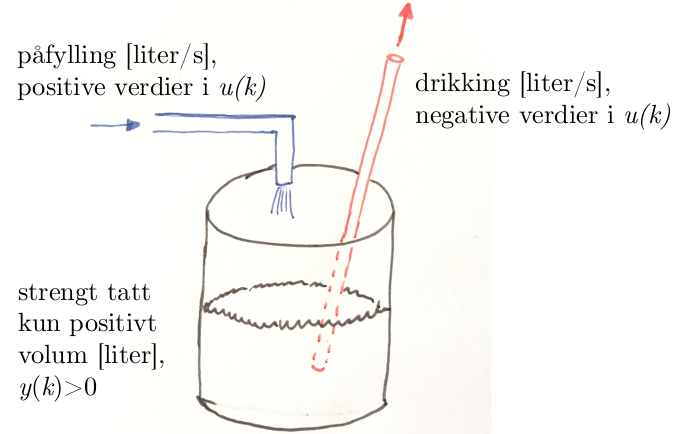
\includegraphics[width=0.8\textwidth]{kap1_skisse_glass.png}
    \caption{Skisse av fylling og tapping av væske fra et glass i et glass. Det kan fylles væske i glasset fra en kran, og væske kan tappes via et sugerør. Hentet fra \citetitle{Dre2023Lego} av \Citeauthor{Dre2023Lego}, \citeyear*{Dre2023Lego}, s. 7.}
    \label{fig:kap1_skisse_glass}
\end{figure}

\end{document}